\section{Stanley-Reisner环}

\subsection{Epi-Mono mapping}
\begin{definition}
 如果 $P, Q$ 是偏序集,那么 $f: P \to Q$ 称为是\textbf{保序的}或\textbf{单调的},如果
$ x < y \implies f(x) < f(y). $
$f: P \to Q$ 称为(偏序集间的)\textbf{同构},如果 $f$ 是双射,并且 $f$ 和 $f^{-1}$ 都是保序映射。
\end{definition}\label{Ehrhart1}

令$[n] = \{1, 2, \ldots, n\}$, $I \subseteq [n]$,$|I| = m$.
那么我们有一下两个结论\\
$\bullet$保序的单射 $\iota: I \rightarrow [n]$的个数为:$\binom{n}{m}$,\\
$\bullet$ 保序的满射 $\pi: [n] \rightarrow I$的个数为:$\binom{n-1}{m-1}。 $  

\begin{example}
设 $ n = 5 $,且 $ I = \{2, 4\} $。\\
所有保序的单射的个数为:$\binom{5}{2} = 10。$\\
所有保序的满射的个数为:$\binom{4}{1} = 4。$
\end{example}

\subsection{Simplicial complex and multicomplex}
Simplicial Complex(单纯复形) 是拓扑学和组合数学中的一个重要概念,用于描述空间的离散结构。它由点、线段、三角形、四面体等更高维的“单纯形”组成,并且满足一定的组合性质。

\begin{definition}
一个单纯复形(也可简称复形 complex) $\mathcal{K}$ 是单纯形的集合,且满足:
\begin{enumerate}
    \item 若单纯形属于 $\mathcal{K}$,则其任意面都属于 $\mathcal{K}$,
    \item 若 $\sigma_1, \sigma_2$ 为 $\mathcal{K}$ 中的两个单纯形,则 $\sigma_1 \cap \sigma_2$ 是空集或者是 $\sigma_1, \sigma_2$ 共有的一个面。
\end{enumerate}
\end{definition}
简而言之,单纯复形就是向下封闭的集合的子集族。\\
令 $\Delta$ 是顶点集 $V = \{x_1, \ldots, x_n\}$ 上的一个有限单纯复形。这意味着 $\Delta$ 是 $V$ 的子集集合,使得如果 $F \subseteq G \in \Delta$,则 $F \in \Delta$,且对于所有 $x_i \in V$,$\{x_i\} \in \Delta$。$\Delta$ 的元素称为面(faces)。如果 $F \in \Delta$,则定义 $\dim F := |F| - 1$,并定义 $\dim \Delta := \max_{F \in \Delta} (\dim F)$。令 $d = \dim \Delta + 1$。给定任意域 $k$,我们现在定义 $\Delta$ 的面环(face ring)或斯坦利-赖斯纳环(Stanley-Reisner ring),记作 $k[\Delta]$。

\begin{definition}
$k[\Delta] = k[x_1, \ldots, x_n]/I_\Delta$,其中
$I_\Delta = \{x_{i_1} x_{i_2} \cdots x_{i_r} \mid i_1 < i_2 < \cdots < i_r,\quad \{x_{i_1}, x_{i_2}, \ldots, x_{i_r}\} \notin \Delta\}。$
\end{definition}

\begin{theoreminner}
$ \dim k[\Delta] = 1 + \dim \Delta = d。 $
\end{theoreminner}

\begin{theoreminner}
定义 $\deg x_i = 1$。那么
\begin{align}
H(k[\Delta], m) = \begin{cases} 
1, & m = 0 \\
\sum _{i=0}^{d-1}f_i \binom{m-1}{i}, & m > 0 
\end{cases}
\end{align}
等价地
\begin{align}
F(k[\Delta], \lambda) = \sum_{i=-1}^{d-1} \frac{f_i \lambda^{i+1}}{(1 - \lambda)^{i+1}}。
\end{align}
\end{theoreminner}


\begin{remark}
表达式 $\sum f_i \binom{m-1}{i}$ 在 $m = 0$ 时给出 $\Delta$ 的欧拉特征。因此,$k[\Delta]$ 的 Hilbert 函数在 $\chi(\Delta) = 1$ 时没有异常值。为了证明上述定理,最简单的方法是先使用更精细的分级,然后再进行特化。定义 $k[\Delta]$ 的精细分级为 $\deg x_i = (0, \ldots, 0, 1, 0, \ldots, 0) \in \mathbb{Z}^n$,其中 $i$ 是单位坐标向量。令 $x_1^{a_1} x_2^{a_2} \cdots x_n^{a_n} = \{x_i \mid a_i > 0\}$。显然,所有形如 $u = x_1^{a_1} x_2^{a_2} \cdots x_n^{a_n}$ 且 $u \in \Delta$ 的单式 $u$ 形成 $k[\Delta]$ 的 $k$-基。通过计算这些单式的支撑 $F \in \Delta$,我们得到精细分级的 Hilbert 系列的以下表达式:
\begin{align*}
 F(k[\Delta], \lambda) = \sum_{F \in \Delta} \prod_{x_i \in F} \frac{\lambda_i}{1 - \lambda_i}。
\end{align*}
\end{remark}

\begin{definition}
$(d-1)$维单纯复形的$f$-向量就是它的各维面的个数$f=(f_{-0}, f_{-1}, \cdots, f_{-(d-1)})$,$f_{-0}$就是其顶点数,$f_{-1}$就是边的个数,$\cdots$,$f_{-(d-1)}$就是其极大面积的个数。
\end{definition}

\begin{definition}
$\Delta$的Euler数定义为$e(\Delta)=f_{-0}-f_{-1}+f_{-2}\cdots+(-1)^{(d-1)}f_{-(d-1)}$
\end{definition}

由此可以计算$k[\Delta]$的($Z^n$分次的)Hilbert多项式
\begin{align*}
H_k[\Delta](t)& = \sum _{F \in \Delta} \sum_{a \in N^n, \text{supp}(a)=F} t^a\\
&=\sum_{F \in \Delta}\prod _{v_i \in F} \frac{t_i}{(1-t_i)}\\
&= \sum_{i=0}^{d-1} f_{-i} \frac{t^{i+1}}{(1-t)^{i+1}}。
\end{align*}

\begin{definition}
对于Stanley-Reisner环,我们有所谓的$h$-向量,它是通过其Hilbert多项式定义如下:
\begin{align*}
H_k[\Delta](t) = h_0 + h_1 t + \cdots + \frac{t^d}{(1-t)^d}。
\end{align*}
\end{definition}

比较上述两式,可以得到$f$-向量与$h$-向量之间的关系:
\begin{align*}
\sum h_i t^i = \sum_{i=0}^{d-1} f_{-(i-1)} \frac{t^i}{(1-t)^{d-i}}
\end{align*}
那么有
\begin{align*}
h_j = \sum _{i=0, \cdots, j} (-1)^{(j-i)} \binom{d-i}{j-i} f_{-(i-1)},
\end{align*}
和
\begin{align*}
f_{-(j-1)} = \sum _{i=0, \cdots, j} \binom{d-i}{j-i} h_i。
\end{align*}
特别地,我们可以得到几个容易计算的公式:
\begin{align*}
h_0 = 1, \quad h_1 = f_{-0} - d, \quad h_d = (-1)^{(d-1)} e(\Delta),
\end{align*}
以及
\begin{align*}
&\sum _{i=0, \cdots, d} h_i = f_{-(d-1)}。
\end{align*}
其中$e(\Delta) = e(\Delta)-1$是$\Delta$的约化Euler数,也可以视为$\Delta$的约化上同调的交错和。

\begin{theoreminner}
向量 $(f_0, f_1, \ldots, f_{d-1}) \in \mathbb{Z}^d$ 是某个 $(d-1)$-维单纯复形 $\Delta$ 的 $f$-向量当且仅当
\begin{align*}
0 < f_{i+1} \leq f_i^{(i+1)}, \quad 0 \leq i \leq d-2。
\end{align*}

\end{theoreminner}


与单纯复形一起,我们还需要多重复形的更一般概念。一个多重复形 $\Gamma$ 在顶点集 $V = \{x_1, \ldots, x_n\}$ 上是一个单式集合 $x_1^{a_1} \cdots x_n^{a_n}$,使得 $u \in \Gamma$,$v | u$ 意味着 $v \in \Gamma$。因此,单纯复形对应于平方自由单式的特殊情况。多重复形有时被拓扑学家称为“半单纯复形”。对于一个多重复形 $\Gamma$,令 $h_i := \# \{u \in \Gamma \mid \deg u = i\}$,并定义 $h$-向量 $h(\Gamma) = (h_0, h_1, \ldots)$。$h$-向量可能是无限的,如果 $\Gamma \neq \emptyset$,那么 $ h_0 = 1 $。

\begin{definition}
如果 $ h_i = 0 $ 对于 $ i > d $,我们也写 $ h(\Gamma) = (h_0, \ldots, h_d) $。序列 $ (h_0, h_1, \ldots) $ 是某个非空多重复形 $\Gamma$ 的 $ h $-向量,称为 $ M $-向量。
\end{definition}

\begin{theoreminner}
$ (h_0, h_1, \ldots) $ 是一个 $ M $-向量当且仅当 $ h_0 = 1 $ 并且 $ 0 \leq h_{i+1} \leq h_i^{(i)}, i \geq 1 $。
\end{theoreminner}

\subsection{Simplicial polytope}

\begin{definition}
在几何学中,一个单纯形(simplicial polytope)是一个三角形或四面体的概念向任意维度的推广。命名为单纯形是因为它表示任意已知维度中最简单的多面体 (polytope)。具体来说,一个$k$ 维单纯形就是一个$k$维多面体,即是其 $(k+1)$ 个顶点的凸包。
\end{definition}
\begin{example}
一个0维单纯形(0-dimensional)是一个点。\\
一个1维单纯形(1-dimensional)是一条线段。\\
一个2维单纯形(2-dimensional)是一个三角形。\\
一个3维单纯形(3-dimensional)是一个多面体。\\
一个4维单纯形(4-dimensional)是一个5点细胞体(5-cell)。
\end{example}

\begin{remark}
Polytope 是一种高维的几何对象,它是通过有限个平面切割空间而得到的一个有界集合。简单来说,它是一个在任意维度上都有明确边界的形状。在一维中,它是一条线段;在二维中,它是多边形;在三维中,它是多面体;在更高维度中,则是相应的高维形式。它的特点是有顶点、边、面等不同维度的“面”,这些面按照一定的规则组合在一起。\\
Simplicial complex 是由多个单纯形(如点、线段、三角形、四面体等)组成的结构,其中每一个单纯形的边界也是该结构的一部分,并且两个单纯形要么不相交,要么只在其公共面(可能是点)上相交。单纯复形可以用来构建更复杂的形状,不仅限于凸形或连通的空间,而且可以在任何维度上定义。\\
Simplicial polytope 是一种特殊的 polytope,它的所有面都是单纯形。换句话说,在 simplicial polytope 中,每个面(包括其自身)都可以被表示为一个单纯形。\\
polytope 是一个广泛的概念,适用于任意维度的有界几何对象;simplicial complex 是由单纯形组成的结构,可用于表示各种复杂形状;而 simplicial polytope 则是一种特殊类型的 polytope,其所有面都必须是单纯形。他们的关系如下图所示:

\begin{figure}[H] % [H] 表示强制当前位置
    \centering
    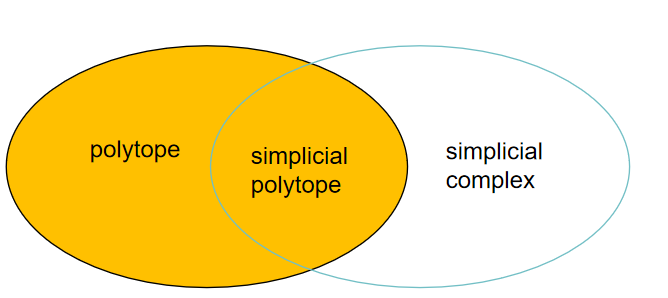
\includegraphics[width=0.5\textwidth]{关系图.png} % 替换 "image.png" 为你的图片文件名
    \caption{关系图} % 图片标题
    \label{fig:my_image} % 图片标签,用于引用
\end{figure}
\end{remark}


\subsection{Stanley-Reisner环}

\begin{definition}
设 $k$ 是作为系数的交换环,给定任何一个顶点集为 $\{v_1, \ldots, v_n\}$ 的单纯复形 $\Delta$,$\Delta$ 关于 $k$ 的 Stanley-Reisner 环是指商 $k$-代数:
$ k[\Delta] = k[x_1, \ldots, x_n] / I_\Delta $
其中 $I_\Delta$ 是由所有使得不属于 $\Delta$ 的单形 $\langle v_{i_1} \cdots v_{i_k} \rangle$ 所对应的单项式 $x_{i_1} \cdots x_{i_k}$ 生成的理想,也称为 Stanley-Reisner 理想。
即$ I_\Delta = [m; m \notin \Delta] $。
\end{definition}
把 $k[\Delta]$ 看作是由各维度上的向量空间组成的直和,则有:
$k[\Delta]=\bigoplus_{i=0}^{\infty} (k[\Delta])_i。$

\subsection{Hilbert 函数}
\begin{definition}
对于每个非负整数 $i$,定义 $k[\Delta]$ 的 Hilbert 函数 $h_{k[\Delta]}(i)$ 为:
$ h_{k[\Delta]}(i) = \dim_k ((k[\Delta])_i) $
这里 $(k[\Delta])_i$ 表示 $k[\Delta]$ 中次数为 $i$ 的部分。
\end{definition}

\section{h-vectors}
\subsection{$Hilbert$级数 }
先回顾前面的知识。\\
在$[n]$上给定一个单纯复形$\Delta$,假设$\Delta$的维数$dim \Delta =d-1$,那么对应的哈斯图($Hasse$)最上面一层代表$\Delta$极大面个数有$d$个。给定任意域 ${\mathbb{K}}$,则$\Delta$的面环(face ring)为$\mathbb{K}[\Delta] =\mathbb{K}[x_1, x_2, \ldots, x_n]/I_\Delta$,其中
$I_\Delta =\{x_{\tau}\ ,\tau \notin \Delta\}$为一个理想。
\begin{lemma}
若$f: \mathbb{N} \rightarrow \mathbb{C}$,$d \in \mathbb{N}$,则有
\begin{align}
\sum_{n=0}^{\infty}f(n)x^{n}=\frac{P(x)}{(1-x)^d}.
\label{eq1}
\end{align}
这里,$P(x) \in \mathbb{C}[x]$,$deg(P) \leq d$。
\end{lemma}

\begin{df}
若 $\Delta$ 的面环 $\mathbb{K}[\Delta]$ 存在,那么它的Hilbert 级数为
\begin{align}
F(\mathbb{K}[\Delta],z)&=\sum_{i=0}^{\infty}(dim\mathbb{K}[\Delta]_{i})z^{i}\nonumber \\[0.5ex]
&=\sum_{i=0}^{\infty}M_{i}z^{i}\nonumber \\[0.5ex]
&=\frac{h_{0}+h_{1}+h_{2}z^2+...+h_{d}z^{d}}{(1-z)^d}.\label{eq2}
\end{align}
其中(Stanley),
\begin{align}
M_{i} = \begin{cases}
1, & m = 0 \\
\sum_{i=0}^{d-1} f_j \binom{i-1}{j}, & m > 0.
\end{cases} \label{eq3}
\end{align}
这里\,$f_{j}$ 是$\Delta$中$j$-维单形的数量。
\end{df}\label{Ehrhart1}

可以发现,为了得到定义\,(\ref{eq2}) 式右边,首先要得到单纯复形$\Delta$每一层的维数公式\,$M_{i}$,再由引理\,(\ref{eq1}) 式推导得到。\par
$M_{i}$ 的理解如之前所讲,对于如下图\ref{fig1}的一个$\Delta$,
\begin{figure}[H] % [H] 表示强制当前位置
\centering % 关键命令:使内容居中
    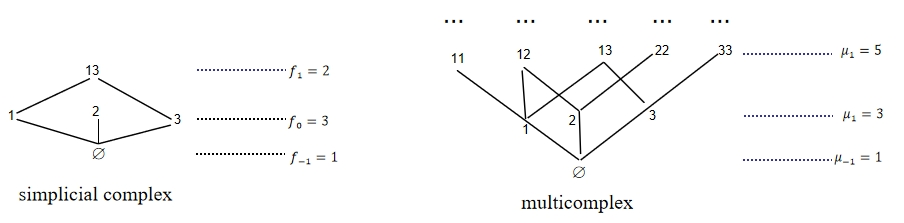
\includegraphics[width=1.2\textwidth]{tupianyi.png}
    \caption{由单纯复形张成的多重复形的例子}% 图片标题
    \label{fig1} % 图片标签,用于引用
\end{figure}
\noindent 所得到的多重复形正好是$Stanley-Reisner$ $ring$每一层向量空间的积。\par
多重复形(图\ref{fig1}右边)的第一层表示向量乘积$x_{1}$,$x_{2}$,$x_{3}$,第二层表示向量乘积 $x^{2}_{1}$,$x_{1}x_{2}$,$x_{1}x_{3}$,$x^{2}_{2}$,$x^{2}_{3}$。$Stanley$ 公式表示的是要数多重复形某一层到底有多少个元素,换言之,即要数某一层向量空间的积的个数,而多重复形的维数可以由它对应的单纯复形的面向量($face$ $vectors$)表示出来,这意味着,当从偏序集的角度来看时,图\ref{fig1}右边可以进行横向拆分(每一层如何由前一层生成)。综上所述,给定一个$\Delta$,构造出它的面向量,就可以得到其$Hilbert$级数。

\subsection{h-vectors }

如果不借助第一节所述分解机制,能否由定义直接得到\,$h-vectors$或者$Hilbert$ 多项式,也就是直接得到\,(\ref{eq2})式最右边的结果。
\begin{df}
将\,$h=(h_{0},h_{1},h_{2},...,h_{d})$ 称为单纯复形\,$\Delta$ 的\,$h-vector$。
\end{df}\label{Ehrhart2}
通过一个例子再次理解\,$h-vector$ 的含义。
\begin{example}
如图$\,\ref{fig2}$ 的 $\Delta$ \par
\begin{figure}[h]
\centering
  % Requires \usepackage{graphicx}
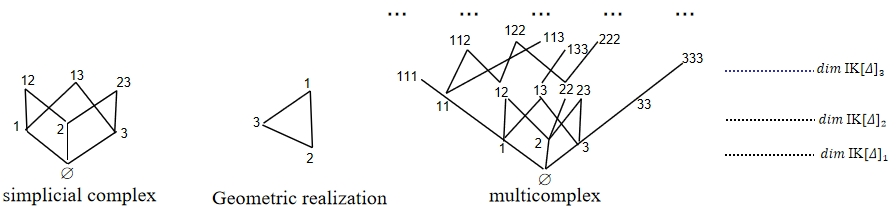
\includegraphics[width=1.2\textwidth]{tupianer.png}
\caption{单纯复形及其多重复形}
\label{fig2}
\end{figure}
\noindent $dim \mathbb{K}[\Delta]]_{i}$表示多重复形每一层向量空间积的个数。那么,它所对应的\,$Hilbert$ 级数为
\begin{align}
F(\mathbb{K}[\Delta],z)&=\sum_{i=0}^{\infty}(dim\mathbb{K}[\Delta]_{i})z^{i}\nonumber \\[0.5ex]
&=1 + 3z +6 z^{2} + 9 z^{3} + 12 z^{4}+... \nonumber \\[0.5ex]
&=\frac{h(z)}{(1-z)^2}. \label{eq4}
\end{align}
\end{example}
(\ref{eq4}) 式右边\,$\frac{h(z)}{(1-z)^2}$ 表示选不同面(face)张成的多重复形对应的生成函数。当遍历\,$\Delta$ 所有的面时,多重复形的纵向分解完成,得到完整的\,$Hilbert$ 级数。\\

\begin{example}
图$\,\ref{fig3}$ 中的的两条射线对应的生成函数可以写成
\begin{align}
1+x+x^2+x^3+x^4+...=\frac{1}{1-x},~~~~~~~
x^4+x^5+x^6+x^7+x^8+...=\frac{x^4}{1-x}
\label{eq5}
\end{align} 
\begin{figure}[h]
\centering
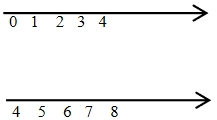
\includegraphics[width=0.3\textwidth]{tupiansi.png}
\caption{平面上射线的例子}
\label{fig3}
\end{figure}
\end{example}

(\ref{eq5}) 式分子部分的不同表示第二条射线与第一条射线相比向右平移了4个单位长度。类似地,在二维空间的也有相同的结,(\ref{eq4}) 式右边的理解也如此。

\begin{df}
对一个单纯复形$\Delta$,任选一个它的面$\sigma$,则$M_{\sigma}=\{\mu \mid support(\mu)=\sigma\}$.
\end{df}

如图\,\ref{fig2} 选\,$\sigma=13\in\Delta$,则\,$M_{\sigma}=\{13, 113, 133, 1113, 1133, 1333,...\}$。

\begin{theoreminner}
若$\sigma=\{i_{1},i_{2},i_{3},...,i_{s}\}\in \Delta$,$M_{\sigma}:=\{x_{\sigma}=x^{\alpha_{1}}_{i_{1}}x^{\alpha_{2}}_{i_{2}}x^{\alpha_{3}}_{i_{3}}...x^{\alpha_{s}}_{i_{s}}\mid\sigma\in\Delta,\alpha_{i}\in\mathbb{Z}_{>0}\}$,
则
\begin{align}
\sum_{\mu\in M_{\sigma}}z^{deg(\mu)}=\prod_{\pi_{j}\in\sigma}(\sum_{d_{j}=1}z^{\alpha_{j}})=\frac{z^{s}}{(1-z)^{s}},
\label{eq6}
\end{align}
遍历\,$\Delta$ 中所有的面
\begin{align}
F(\mathbb{K}[\Delta],z)&=\sum_{\sigma\in\Delta}\frac{z^{\mid\sigma\mid}}{(1-z)^{\mid\sigma\mid}} \label{eq7}\\
&=\sum_{i=0}^{d}f_{i-1}\frac{z^{i}}{(1-z)^{i}} \label{eq8}\\
&=\sum_{i=0}^{d}f_{i-1}\frac{z^{i}(1-z)^{d-i}}{(1-z)^{d}} \label{eq9}\\
&:=\frac{\sum_{i=0}^{d}h_{i}z^{i}}{(1-z)^{d}}.
\label{eq10}
\end{align}
\end{theoreminner}

(\ref{eq7}) 式是对\,$\Delta$ 面的加和,(\ref{eq8}) 式是对其多重复形维数的加和,(\ref{eq9}) 式为多重复形\,$d-1$ 的形式,(\ref{eq10}) 式明确了\,$h_{i}$ 和\,$h-vector$ 的关系,即
\begin{align}
\sum_{i=0}^{d}f_{i-1}z^{i}(1-z)^{d-i}&=f_{-1}(1-z)^{d}+f_{0}z(1-z)^{d-1}+...+f_{d-1}z^{d}\nonumber \\[0.5ex]
&=h_{0}+h_{1}z+...+h_{d}z^{d}. \label{eq11}
\end{align}

\subsection{Stanley's  trick }
介绍一种由\,$f$ 向量直接得到\,$h$向量的技巧。\\

\begin{df}
给一个\,$\Delta$,有\,$f={f_{0},f_{1},f_{2},...,f_{d-1}}$ 。\par
\begin{figure}[h]
\centering
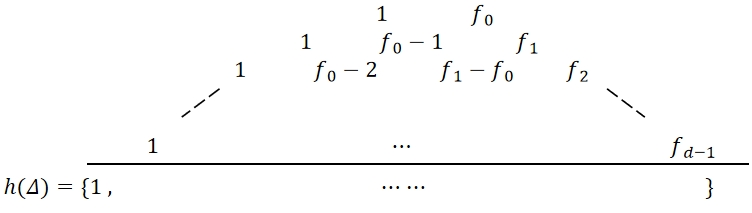
\includegraphics[width=0.8\textwidth]{tupianwu.png}
\caption{Stanley's \,trick}
\label{fig4}
\end{figure}
\end{df}

将表格 \,\ref{fig4} 的左上角至右下角依次写\,$f$ 向量,右上角至左下角全部标为\,$1$,此后每一行的量由上一行与之相邻的右侧量与左侧量做减法得到,表格最底部的量即是\,$\Delta$ 对应的\,$h$ 向量。

从矩阵的角度来考虑\,$f$ 向量和\,$h$ 向量的关系。
\begin{theoreminner}
如果将\,$\Delta$ 对应的\,$f$ 和\,$h$ 向量按倒序写成列向量的形式,那么与定义等价的矩阵表达形式为
\begin{equation}  \label{eq3.12}
\left[
\begin{array}{cccccc} % 6列均居中对齐(c: center)
\binom{0}{0} & \binom{1}{0} & \binom{2}{0} & ... & \binom{d-1}{0} & \binom{d}{0} \\ % 第1行
\binom{0}{1} & \binom{1}{1} & \binom{2}{1} & ... & \binom{d-1}{1} & \binom{d}{1} \\ % 第2行
... & ... & ... & ... & ... & ... \\ % 第3行
\binom{0}{d-1} & ... & ... & ... & \binom{d-1}{d-1} & \binom{d}{d-1} \\ % 第3行
\binom{0}{d} & \binom{1}{d} & \binom{2}{d} & ... & \binom{d-1}{d} & \binom{d}{d}    % 第4行(最后一行不加\\)
\end{array}
\right]
\left[
\begin{array}{ccccc}
h_{d}\\
h_{d-1}\\
... \\
h_{1} \\
h_{0} \\
\end{array}
\right]=
\left[
\begin{array}{ccccc}
f_{d-1}\\
f_{d-2}\\
... \\
f_{0} \\
f_{-1} \\
\end{array}
\right],
\end{equation}
其中,二项式系数\,$\binom{i}{j}$,\,$0\leq i\leq d, 0\leq j\leq d$,分别为矩阵的列指标和行指标。将
\begin{equation}  \label{eq3.12}
M=\left[
\begin{array}{cccccc} % 6列均居中对齐(c: center)
\binom{0}{0} & \binom{1}{0} & \binom{2}{0} & ... & \binom{d-1}{0} & \binom{d}{0} \\ % 第1行
\binom{0}{1} & \binom{1}{1} & \binom{2}{1} & ... & \binom{d-1}{1} & \binom{d}{1} \\ % 第2行
... & ... & ... & ... & ... & ... \\ % 第3行
\binom{0}{d-1} & ... & ... & ... & \binom{d-1}{d-1} & \binom{d}{d-1} \\ % 第3行
\binom{0}{d} & \binom{1}{d} & \binom{2}{d} & ... & \binom{d-1}{d} & \binom{d}{d}    % 第4行(最后一行不加\\)
\end{array}
\right].
\end{equation}
称为由\,$h$ 向量到\,$f$ 向量的过渡矩阵。
\end{theoreminner}
注意,矩阵\,$M$ 与其过渡矩阵\,$M^{-1}$ 有相同的表达形式。尽管\,$h$ 向量和\,$f$ 向量可以相互推导,但在研究过程中,学者们更关注\,$h$ 向量。

\subsection{Dehn-Sommerville Relation }
\begin{df}
如果\,$\Delta$是一个单纯球体 (simplicial sphere),则
\begin{align}
h_{i}=h_{d-i}.
\label{eq14}
\end{align}
\end{df}

\begin{example}
$h_{0}=f_{-1}$,\par
$h_{d}=f_{d-1}-f_{d-2}+...+f_{-1}$,\par
由\,$h_{0}=h_{d}$,得到\,$f_{d-1}-f_{d-2}+...-f_{0}+(-1)^{d}f_{-1}=f_{-1}$,
整理得到欧拉示性数($Euler \,characteristic$),$\chi(\Delta)=f_{0}-f_{-1}+f_{2}+..+f_{d-1}=0$。
欧拉示性数描述了\,$f$ 向量的一个线性关系,而$\,h_{i}=h_{d-i}$ 描述了\,$\Delta$ 的$\frac{d}{2}$个线性关系。
\end{example}
\begin{df}
给定一个$\,\Delta$,则它对应的\,$g$ 向量为
\begin{align}
g_{i}=h_{i}-h_{i-1}.
\label{eq15}
\end{align}
\end{df}
